\section{АНАЛІЗ АЛГОРИТМІВ РЕКОМЕНДАЦІЙ}
Моделі і алгоритми глибокого навчання на основі штучних нейронних мереж в останні роки знаходять своє використання у багатьох прикладних сферах інформатики. Цей підхід також показав прекрасні результати у порівнянні із класичними моделями у задачах побудови рекомендацій, що є наслідком уміння нейромереж знаходитити не лінійні і не тривіальні зв’язки у навчальних даних. А також, можливість використання в якості джерела даних як візуальну, так і текстову, контекстну інформацію.

\begin{figure}[H]
    \centering
    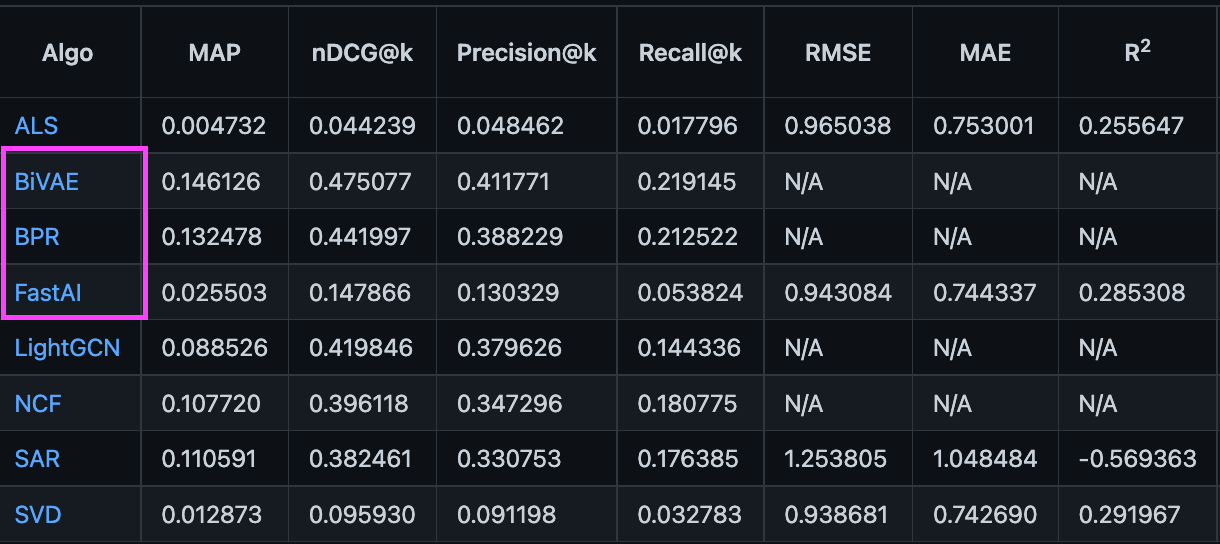
\includegraphics[width=0.8\textwidth]{images/NN_model_res.png}
    \caption{Порівняльні результати роботи моделей на основі нейромереж}
\end{figure}


Для практичних експериментів було обрано актуальні алгоритми рекомендацій які були представлені у останні декілька років. Із інших критеріїв було взято до уваги популярність у науковій сфері і використання у практичних реалізаціях.

Також, кожна розглянута модель відповідає певній групі алгоритмів для нейромережевої побудови рекомендацій.

\subsection{Алгоритм Neural Collaborative Filtering}

\begin{figure}
    \centering
    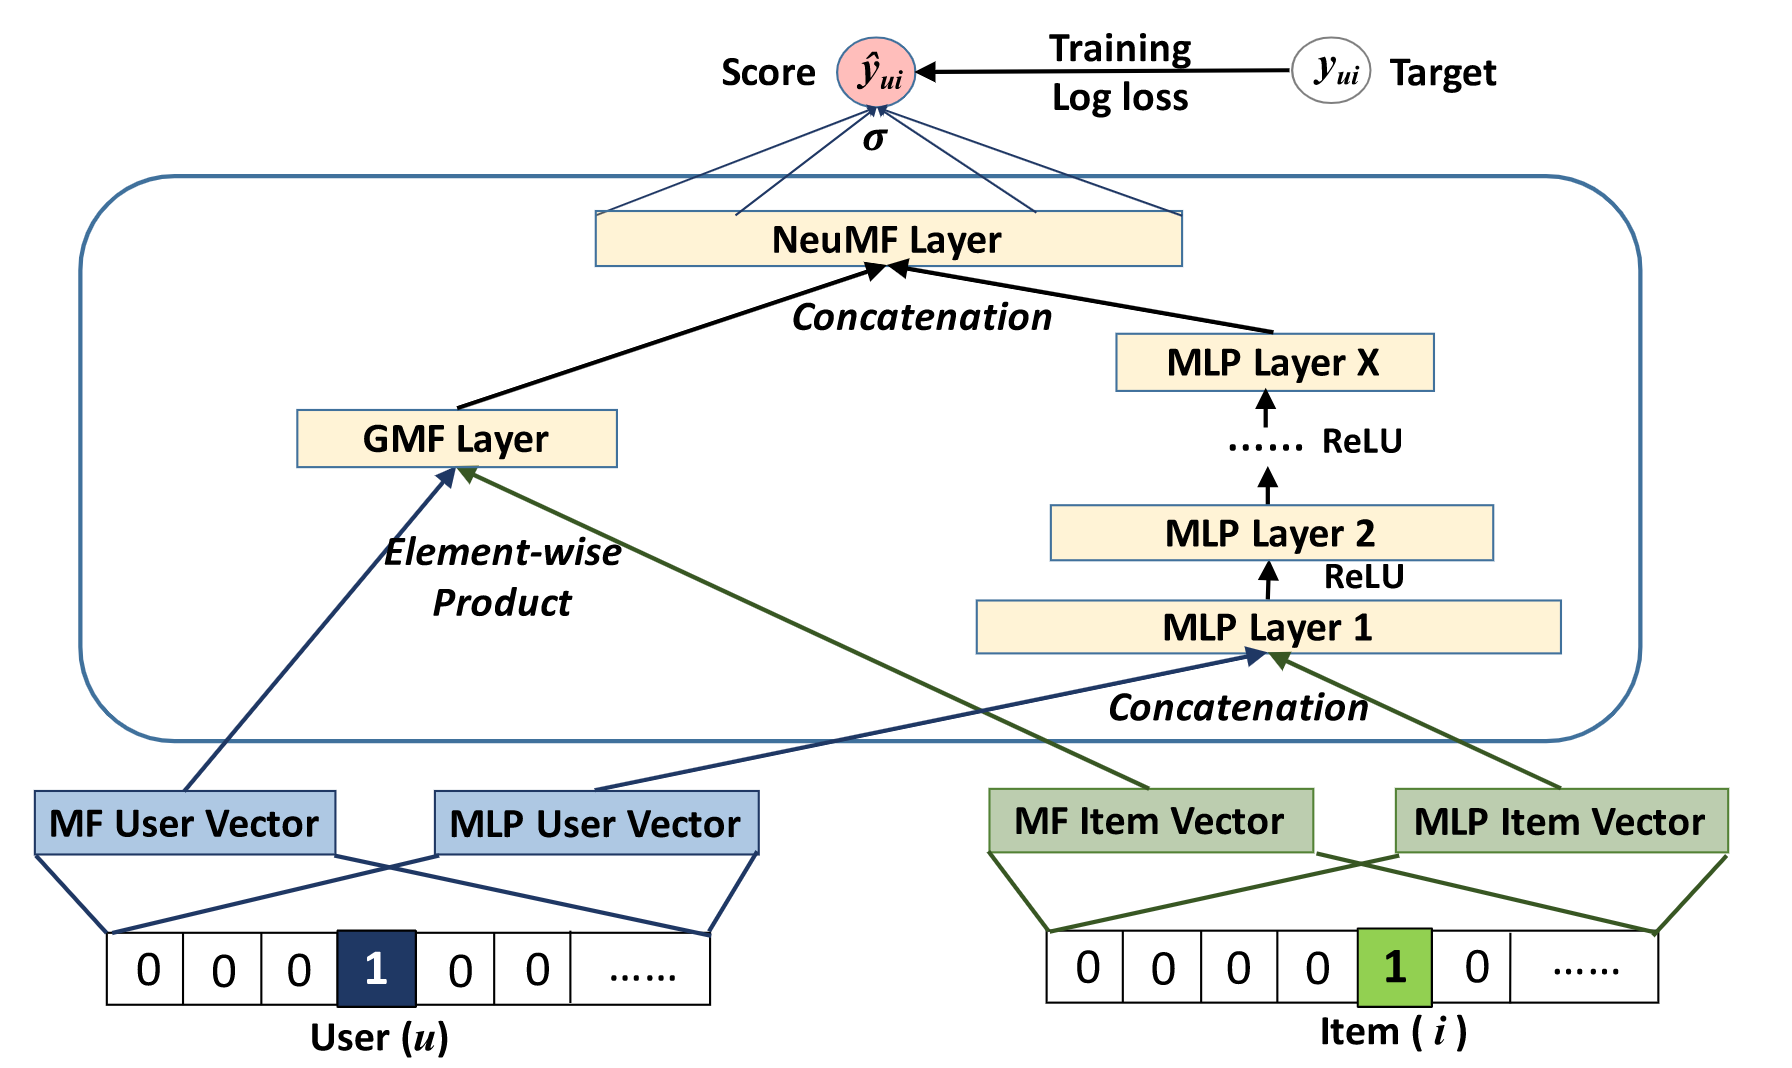
\includegraphics[width=0.8\textwidth]{images/NCF.png}
    \caption{Умовна будова NCF}
\end{figure}

Алгоритм нейронної факторизації NCF є потужним поєднанням алгоритму нейронної факторизації і багатошарового персептрону. Такий сплав лінійного і нелінійного підходу показує свою високу єфективність у моделюванні прихованих  взаємозв’язків між користвучем і об’єктом.

У звичайній матричній факторизації усі елементи знаходяться у одному прихованому просторі, що надає нам можливість визначити схожість між потрібними нам векторами використовуючи скалярний добуток/подібність косинуса або коефіціент Жаккара. Під матричною факторизацією маємо на увазі наступну модель оцінки взаємодії:
\[\hat{y}_{ui} = f(u,i|p_{u},q_{i}) = p^{T}_{u}q_{i} = \sum_{k = 1}^{K}p_{uk}q_{ik}\]

Але у задачах рекомендацій із неявною взаємодією (impicit feedback)
виникають проблеми із обрахуванням схожості внаслідок обмежень.

\begin{figure}
    \centering
    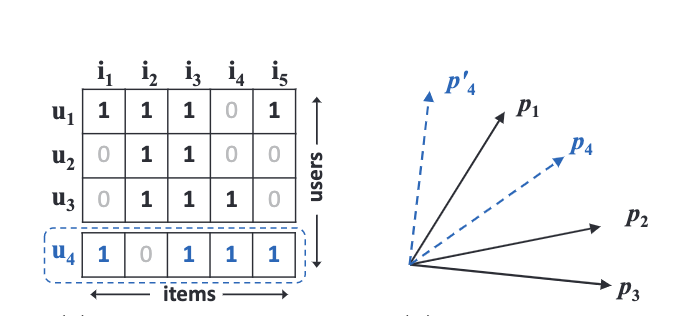
\includegraphics[width=0.8\textwidth]{images/MF_limitation.png}
    \caption{Зліва - матриця взаємодій користувача/об’єкта.Справа відображення у прихований простір. Положення вектора p4 відносно p3 ілюструє обмеженність. (Схожість p4 до p3 вища ніж до p2 але оптимально виразити ми не можемо).  }
\end{figure}

На вхід моделі подаються ембедінги користувача і об’єкта відповідно. Ці бінаризовані вектори можуть представляти широкий спектр корисної інформації - від вектора взаємодій до зжатих даних про вподобання користувача, історію або додаткову інформацію про об’єкт. Така особливість нівелює проблему холодного старту.

GMF(Generalized Matrix Factorization) - частина моделі яка відповідає за нейронну матричну факторизацію. Вхідні бінаризовані вектори можна інтерпритувати як приховані змінні користувача - $p_{u}$ і об’єкта відповідно $q_i$. Вхідний вектор що поступає на вхід:
\[\phi_{1}(p_{u}, q_{i}) = p_{u} \odot q_{i}\]
де $\odot$  відповідає за по елементний добуток. Вихідний вектор GMF:
\[\hat{y}_{ui} = a_{out}(h^{T}(p_{u} \odot q_{i}))\]
де $a_{out}$ відповідають за функцію активації і ваги вихідного шару.
При лінійній $a_{out}$ і юніт векторі $h$ відтворюється прямий вихід алгоритму матричної факторизації. Для базової імплеменатації була обрана сигмоїдна функція активації
\[ \sigma(x) = \frac{1}{1 + e^{-x}}\]
та логістична функція втрат.

MLP - використовуєтсья для моделювання не лінійної взаємодії. Це нейронна мережа прямого поширення із вежоподібною структурою (кожен наступний шар має вдвічі меншу розмірність). Формулювання мережі наступне:
\begin{align}
    \mathbf{z}_1 =\phi_1\left(\mathbf{p}_u, \mathbf{q}_i\right)=\left[\begin{array}{c}\mathbf{p}_u \\
                                                                              \mathbf{q}_i\end{array}\right],  \\
    \phi_2\left(\mathbf{z}_1\right) =a_2\left(\mathbf{W}_2^T \mathbf{z}_1+\mathbf{b}_2\right),         \\
    \cdots \cdots                                                                                      \\
    \phi_L\left(\mathbf{z}_{L-1}\right) =a_L\left(\mathbf{W}_L^T \mathbf{z}_{L-1}+\mathbf{b}_L\right), \\
    \hat{y}_{u i} =\sigma\left(\mathbf{h}^T \phi_L\left(\mathbf{z}_{L-1}\right)\right)
\end{align}

де $W_{x}$, $b_{x}$ і $a_{x}$ відповідають матриці вагів, вектору зміщення та функції втрат ReLU. Вибір функції активації обумовлений її властивістю до не насичення і більшою близькою до біологічної структури. Також, відомо що ReLu менш вразлива до перенавчання і є зручної при навчанні на розріджених даних.

Одними із важливих гіперпараметрів моделі є розмір вихідних векторів прихованих змінних. Чим вони більші, тим більш глибоко модель може генералізувати інформації про взаємодію. Тому для імплементації було відібрано декілька їх варіацій.

Фінальним поєднанням двох блоків моделі є шар NeuMF, на якому і обчислюється вихід мережі $\hat{y}_{u i}$. Комбінація результатів MLP і GMF відбувається за рахунок повнозвязного шару на вхід якого подається конкатенація двох векторів прихованих змінних. Використовуючи функцію активації ReLu ми отримуємо таку оцінку:
\begin{align}
    \hat{y}_{u i}=\sigma\left(\mathbf{h}^T\left[\begin{array}{l}
                                                        \phi^{G M F} \\
                                                        \phi^{M L P}
                                                    \end{array}\right]\right)
\end{align}

тут $\mathbf{h}$ це вектор вагів який задає вплив кожного блоку. Також, він може використовуватись для ініціалізації із препідготовлених вагів. Спочатку навчити із випадковомими вагами, а після досягнення збіжності використати ваги для фінального навчання:
\begin{align*}
    \mathbf{h} \leftarrow\left[\begin{array}{c}
                                       \alpha \mathbf{h}^{G M F} \\
                                       (1-\alpha) \mathbf{h}^{M L P}
                                   \end{array}\right]
\end{align*}
До моделювання функції втрат мережі потрібно підходити як до задачі бінарної класифікації (через бінаризацію вхідних даних і implicit формулювання). Тому функції втрат регресії не підходять (MSE  подібні). Значення прогнозувань моделі $y_{u i}=1$ інтерпритуємо, що обє’кт i важливий для u, а при 0, що ні.

Тому ми обмежуємо значення $y_{ui}$ інтервалі від [0, 1]. Додатково, це обмеження дозволяє використати ймовірносний підхід до інтерпритації.
Тоді функція правдоподібності приймає наступний вигляд:
\begin{align}
    p(\mathcal{Y}, \mathcal{Y}^{-} \mid \mathbf{P}, \mathbf{Q}, \Theta_f)=\prod_{(u, i) \in \mathcal{Y}} \hat{y}_{u i} \prod_{(u, j) \in \mathcal{Y}^{-}}(1-\hat{y}_{u j})
\end{align}
де $P \in \mathbb{R}^{M \times  K}$ і $Q \in \mathbb{R}^{N \times K}$ відповідає за матриці прихованих змінних, $\theta_{f}$ за параметри моделі функції взаємозв’язків f.
Наступну функцію потрібно мінімізувати використовуючи одим із бажаних варіантів градієнтного спуску:
\[
    L =-\sum_{(u, i) \in \mathcal{Y} \cup \mathcal{Y}^{-}} y_{u i} \log \hat{y}_{u i}+\left(1-y_{u i}\right) \log \left(1-\hat{y}_{u i}\right) .
\]
\subsection{Алгоритм VAE}

Для кожного користувача $u$ семплюється вектор $z_{u}$ розмірності K із багатовимірного нормального розподілу . K відповіє простору прихованих змінних і вміщує у собі інформацію про ключові структурні особливості об’єкта (у простому випадку для цифр це може бути їх колір, кут нахилу або ширина).
Для кожного вектора прихованих змінних нелінійна функція $f_{\theta}(.) \in \mathbb{R}^{I}$ надає оцінку щільності розподілу для набору  $I$ об’єктів рекомендацій $\pi(z_{u})$:
\begin{equation}
    z_u \sim \mathcal{N}(0, I_K), \pi(z_u) = softmax\{f_\theta(z_u)\}, x_u \sim Mult(N_u, \pi(z_u))
\end{equation}

У якості нелінійної функції виступає багатошаровий персептрон із параметрами $\theta$. Вихід цієї трансформації нормалізується функцією softmax і повертає
ймовірносний вектор $\pi(z_u)$ який містить значення для кожного об’єкту рекомендацій. Припускаємо що вектор $x_u$ належить поліноміальному розподілу із ймовірністю  $\pi(z_u)$. Функція правдоподібності для користувача $u$ відносно його прихованого відображення, нагороджує модель збільшуючи ймовірність ненульових елементів $x_u$:
\[ \log p_{\theta}(x_u|z_u) = \sum_i x_{ui} \log \pi_i(z_u)\]
Але через обмеженість $\pi(z_u)$, який сумується до одиниці, модель змушена підвищувати ймовірність на об’єктах які більш правдоподібно будуть обрані користувачем.
\begin{figure}
    \centering
    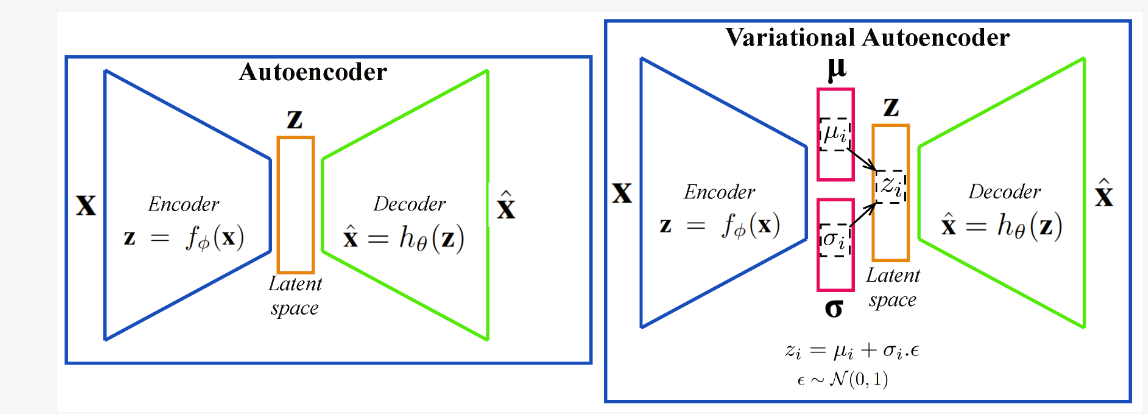
\includegraphics[width=1\textwidth]{images/AE.png}
    \caption{Ілюстративний приклад архітектури AE і VAE.}
\end{figure}
У задачі колаборативної фільтрації розглядають дві функції правдоподібності.
Допустим $f_{\theta}(z_u) \equiv [f_{u1}, \ldots, f_{uI}]^{T}$ є виходом генеративної функції $f_{\theta}(\cdot)$:
\begin{itemize}
    \item Функція правдоподібності Гауса:
          \[\log p_{\theta}(x_u|z_u) = - \sum_i \frac{c_{ui}}{2}(x_{ui} - f_{ui})^{2} \]
    \item Логістична функція:
          \[ \log p_{\theta}(x_u|z_u) = \sum_i x_{ui} \log \sigma(f_{ui} + (1 - x_{ui} \log(1 - \sigma(f_{ui}))))\]
\end{itemize}

Апроксимація $\log p_{\theta}(x_u|z_u)$, через його складність, виконується простішим нормальним розподілом $q(z_u) = \mathcal{N}(\mu_u, \sigma^{2}_u )$ із допомогою методів вараційного аналізу.

Для поняття відстані або відмінності між двома розподілами використовують відстань (дивергенцію) Кульбака-Лейблера. Яка є несиметричної мірою віддаленості один від одного двох ймовірностних розподілів, що задані на спільній множині елементарних подій. Відстань від розподілу $Q$ до $P$  позначається як $D_{KL}(P||Q)$, де $P$ сприймаємо за істинний розподіл, а $Q$ за розподіл який потрібно перевірити. У Теорії Інофрмації використовують інтерпретацію що $D_{KL}(P||Q)$ це кількість втраченої інформації при заміні істини $P$ на розподіл  $Q$:

\[ D_{KL}(P||Q) = \int_X p \log \frac {p}{q}\]

де $p = \frac{dP}{d\mu}$ і $q = \frac{dQ}{d\mu}$ неперервні функції із мірою $\mu$ на $X$.

Тому оптимізація варіаційних параметрів  $\{\mu_u, \sigma^{2}_u\}$ відбувається в наслідок  мінімізації  $ KL (q(z_u)) || p(z_u|x_u) $, яка є частиною функції втрат:
\[  \log p(x_u; \theta) \geq  \mathbb{E}_{q_{\phi}(z_u|x_u)} [ \log p_{\theta} (x_u|z_u)] -  KL (q_{\phi}(z_u|x_u) || p(z_u))  \equiv \mathcal{L}(x_u;\theta, \phi)\]

Цей вираз також відомий як розмір нев’язки або нижньої варіаційної границі (ELBO). Для її знаходження градієнтним спуском використовують так званий reparametrization trick який гарантує неперервність яка необхідна для back propagation. Ми семпюємо із деякого нормального розподілу  $\epsilon \sim \mathcal{N}(0, I_K)$ і модифікуємо $z_{u} = \mu_{\phi}(x_u) + \epsilon \odot \sigma_{\phi}(x_u)$. Що ізолює процесс генерації від пошуку градієнту напряму.
\subsection{Алгоритм Neural Graph Collaborative Filtering}
\begin{figure}
    \centering
    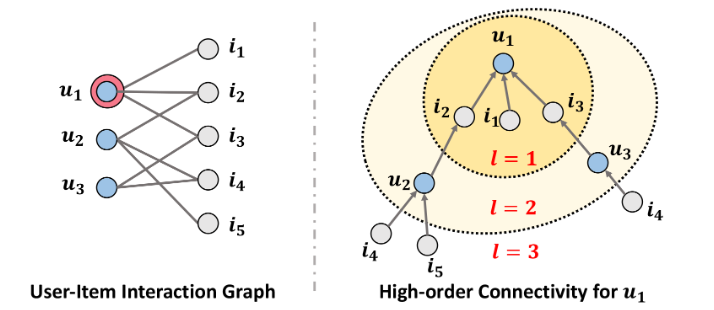
\includegraphics[width=0.8\textwidth]{images/interactions_graph.png}
    \caption{Приклад графу взаємодій користувач-об’єкт, а також ілюстрація взаємодій вищих порядків для NGCF }
\end{figure}
Алгоритм нейромережевої колаборативної фільрації на основі графів використовує підхід інтеграції взаємодій користувач-об’єкт у вигляді дводольного графу.
Такий підхід надає можливість моделювання взаємодій високого порядку, кодуючи у приховане відображення такі складні сигнали як поведінка користувача, що є надзвичайно ефективним у задачах рекомендацій для соціальних мереж.

На Рис 4.5 зображено ієрархію взаємодій для умовного користувача $u_1$. На першому рівні $l_1$ міститься інформація про об’єкти з якими $u_1$ контактував напряму (іншими словами, довжина шляху до яких дорівнює 1) і так далі для кожного наступного рівня (або шару). Використовуючи таку інтерпретацію ми описуємо подібність між користувачами на основі взаємодій. Наприклад ланцюг $u_1 \leftarrow i_2 \leftarrow u_2$ вказує на подібність поведінки $u_1$ і $u_2$ так як вони переглянули об’єкт $i_2$, а аналіз більш довшого шляху $u_1 \leftarrow i_2 \leftarrow u_2 \leftarrow i_4$ пропонує рекомендувати $i_4$ нашому цільовому користувачу $u_1$ ($i_4$ було обрано користувачем $u_2$,  і користувачем $u_3$ додатково).

Головна ідея алгоритму лежить у семплюванні прикладів взаємодій із навчального набору і ітеративного кодування інформації нейронною мережею виконуючи так званий information propagation. Що насичуює латентне відображення потрібною нам інформацією. Модель частково поворює структуру автоенкодера через присутність пари енкодер-декодер. На виході ми отримуємо оцінку релевантності об’єкта рекомендацій для користувача.   

\begin{figure}
    \centering
    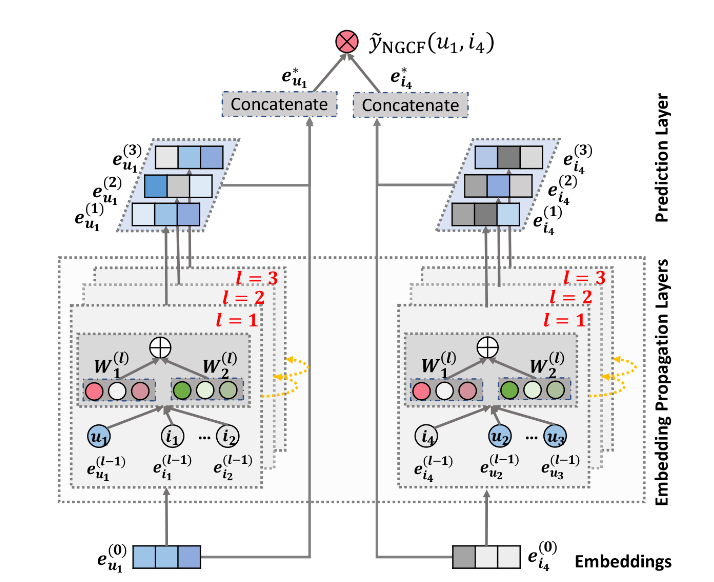
\includegraphics[width=0.8\textwidth]{images/NGCF.png}
    \caption{Архітектура моделі NGCF. Розглянуто приклад побудови оцінки рекомендації $i_4$ для користувача $u_1$}
\end{figure}

Модель складається із трьох компонентів - шару ініціалізації прихованих змінних, групи шарів насичення латентних змінних високорівневою інформацією, і шаром побудови оцінок (prediction). $e_u \in \mathcal{R}^{d}$ і $e_i \in \mathcal{R}^{d}$ вектор прихованих змінних користувача і об’єкта які описують їх поведінку, де $d$ відповідає розміру. Загальна матриця прихованих значень :
\[ E = [e_{u_1},\ldots, e_{u_N}] \times [e_{i_1},\ldots, e_{i_N}] \]. 

У подальшому, ми будемо навчати матрицю $E$ обновлюючи її значення. Цей процес називається агрегацією сигналів (message aggregation), і оперує так званим повідомленням:
\[m_{u \leftarrow i} = f(e_i, e_u, p_{ui})\]
де  $f(.)$ функція кодування повідомлення, що використовує в якості входу наші ембедінги $e_i$ і  $e_u$, $p_{ui}$ відповідає за коефіціент віддаленості для взаємодій і штрафує пропорційно відстані між $u$ до $i$.
Розглядаємо наступну функцію кодування:
\[ m_{u \leftarrow i} = \frac{1}{\sqrt{|N_{u}| |{N_{i}|}}} (W_1e_i + W_2(e_i \odot e_u))\]

Де $W_1$, $W_2$ є матриці вагів нейромережі які відбирають корисну інформацію для передачі. А $\frac{1}{\sqrt{|N_{u}| |{N_{i}|}}}$ відповідає за 
фактор віддаленості.

Зібравши інформацію із кожного сусіда $u$ ми обновлюємо $e_u$ використовуючи функцію активації LeakyReLU (дозволяє малий сигнал у випадку неактивації нейрону): 

\[  e_u = LeakyReLU(m_{u \leftarrow u} + \sum_{i \in \mathcal{N}_u} m_{u \leftarrow i})\]

де LeakyReLU:
\[ LeakyReLU(x) = \begin{cases}
    x, \text{if $x > 0$} \\
    0.01 x
\end{cases}\]
$m_{u \leftarrow u} = W_1 e_u$ відповідає за збереження сигналу із попередніх ітерацій.
\subsection*{Висновки}
Було проаналізовано моделі побудови рекомендацій на основі нейромереж. 
Обрано для експерементального дослідження моделі нейромережевої факторизації, варіаційного автоенкодера і графової колаборативної фільтрації. Для розглянутих алгоритмів було досліджено принцип їх функціонування, архітектуру, функції активацій, моделювання функцій втрат,  наведено інструкції для реалізації.